\section{RELATED WORKS}

    The problem addressed in this work monocular altitude estimation above water surfaces using convolutional neural networks trained on synthetic imagery occupies a notably underexplored niche in the literature.
    While substantial research exists on monocular depth estimation over rigid, textured surfaces \cite{MonocularDepth} \cite{Joglekar2011DepthEU}, and on CNN-based UAV perception for obstacle avoidance \cite{CNNSingleImageQuadrotor} \cite{AircraftColAvoid}, autonomous navigation \cite{ByMySelf}, and object detection and tracking \cite{SurveyObjDetectionTracking} \cite{OpticalFlowStereo}, no prior work has specifically targeted the regression of absolute altitude from a single downward-facing image of a water surface.
    This gap is significant: water surfaces defeat conventional altimetry sensors (LIDAR, ultrasonic, barometric) due to specular reflectivity, surface dynamics, and evaporation-driven barometric drift, yet they remain a critical operational environment for UAVs in offshore inspection, maritime search-and-rescue, and environmental monitoring.
    The contribution of the present work is therefore exclusive in its formulation, combining HSV-based feature extraction, photorealistic synthetic data generation, and CNN-based regression to address a problem for which no existing solution is adequate.

    To contextualize this contribution, the following subsections review the closest related efforts in three areas: CNN-based UAV estimation systems, water surface detection and proximity sensing, and training with synthetically generated datasets.

    \subsection{CNN-Based UAV Estimations}

    Altitude estimation for unmanned aerial vehicles has traditionally relied on processing data from barometers, ultrasonic sensors, and LiDAR through classical filtering algorithms \cite{MonocularDepth}.
    Each technology carries distinct limitations: barometric altimeters suffer from drift due to atmospheric pressure variations; ultrasonic rangefinders fail over surfaces that absorb or scatter acoustic energy; and LiDAR performance degrades severely over specular or semi-transparent surfaces \cite{FiltroKalmanAltitude}.
    Even modern sensor fusion approaches based on Kalman and complementary filters cannot compensate for scenarios in which all constituent sensors produce unreliable readings simultaneously, as occurs over highly reflective surfaces such as water, snow, and sand dunes \cite{WeatherConstraints}.

    The application of CNNs to UAV perception tasks has demonstrated that vision-based approaches can complement or replace traditional sensors in constrained scenarios.
    \cite{OnboardCNN} proposed a seven-layer Single Shot Detection CNN (SSD7) for onboard identification of landing conditions, deployed within a ROS framework on a low-power Intel Stick M3 and achieving 13 fps in real time.
    \cite{ByMySelf} developed a self-supervised system for indoor UAV navigation, where an AlexNet-based architecture processed RGB images fused with infrared and ultrasonic data in a parallel-input configuration. The system outputs a set of navigation options with associated direction and speed for collision avoidance and autonomous flight.
    \cite{MobileNetTracking} proposed a lightweight object tracking model with distance calculation for real-time UAV operation on mobile devices.
    The architecture was based on MobileNet variants (MobileNetv1, MobileNetv2, and E-MobileNet) with seven hidden layers, achieving 56 fps on an NVIDIA Jetson AGX Xavier with an average accuracy of 87.2\%.
    More recently, \cite{VIAENetAltitude} presented VIAE-Net, an end-to-end altitude estimation system that fuses monocular visual features with inertial measurements for UAV autonomous landing, demonstrating the viability of deep learning for metric altitude recovery.

    These works collectively establish that CNNs are capable of extracting spatial and metric information from monocular imagery in UAV contexts.
    However, none of them address the specific challenge of altitude estimation over water, where the absence of stable visual landmarks, the variability of surface texture with wave conditions, and the confounding effects of specular reflection demand a fundamentally different approach.

    \subsection{Water Surface Detection and Proximity Sensing}

    A small but growing body of work has addressed the problem of detecting and characterizing water surfaces from aerial and ground-level imagery, though none have formulated the problem as altitude regression.

    \cite{SAMARANAYAKE2023103933} introduced two techniques for water surface identification from UAV-mounted cameras.
    The first, UNet-RAU, is a segmentation architecture based on UNet with Reflection Attention Units that exploits the specular reflection properties of water to segment water pixels from front-facing camera views, achieving an F1-score of 80.97\% on a custom Drone-Water-Front dataset.
    The second method, Dense Optical Flow based Water Detection (DOF-WD), identifies water surfaces in downward-facing video streams by leveraging rotor downwash-generated ripples at low altitudes and natural texture features at higher altitudes.
    While this work demonstrates that water surfaces can be reliably detected from UAV imagery, including from downward-facing cameras, the task remains binary detection (water vs.\ non-water) rather than metric altitude estimation.
    The present work extends beyond this boundary by treating the water surface not merely as a class to be detected, but as a visual signal from which continuous altitude values can be regressed.

    \cite{ChangXu2024DCUNet} proposed DCU-Net, a dense connection U-Net architecture combining DenseNet-121 and U-Net for water puddle segmentation on road surfaces.
    The model was designed for deployment in IoT-enabled environments and demonstrated improved detection accuracy compared to standard segmentation baselines.
    Although the application domain shares the geometric configuration of a camera perpendicular to a water surface, the objective is semantic segmentation rather than depth or altitude regression.
    Nevertheless, the work confirms that CNN architectures can learn meaningful features from water surface imagery captured in a top-down perspective, which is a relevant finding for the present research.

    \cite{WaterDepthSpecular} addressed self-supervised monocular depth estimation on water scenes by incorporating a specular reflection prior, acknowledging that standard depth estimation methods fail when confronted with the reflective properties of water.
    Their work confirms the central premise of the present thesis: that water surfaces require specialized treatment in vision-based depth and altitude estimation systems.

    \cite{CHEN2022110819} applied CNNs to estimate water surface elevation from laboratory imagery, evaluating Baseline, VGGNet, and ResNet architectures.
    Their results showed that CNN performance is sensitive to the choice of network structure but relatively insensitive to network depth, and that the learned attention hotspots correspond to regions of significant intensity change caused by wave propagation.
    This finding supports the hypothesis of the present work that altitude-related cues are encoded in the texture and brightness patterns of the water surface.

    \subsection{Training with Synthetically Generated Datasets}

    The use of synthetic data for training deep learning models is a well-established practice in domains where real image banks are sparse, expensive to produce, or dangerous to collect \cite{BlenderSmoke} \cite{BlurFiducial} \cite{ObjetoSintetico} \cite{TurbineBlur} \cite{BlenderMapa}.
    This strategy enables safer development cycles, particularly in proof-of-concept stages, by eliminating the need for costly field equipment and prolonged human exposure to hazardous environments.
    In the context of the present work, no open dataset exists containing downward-facing images of water surfaces with associated altitude labels, making photorealistic rendering in Blender not merely convenient but a methodological necessity.

    Several related works illustrate the effectiveness of synthetic data pipelines across diverse domains.
    \cite{TurbineBlur} addressed the problem of motion blur in UAV-captured images of wind turbine blades, for which adequate cataloged images are unavailable.
    They combined three strategies: compositing images of moving and stationary propellers, generating hybrid motion-blurred images through a generative network, and simulating propeller motion to produce virtually blurred images.
    The resulting bank was processed by M-DeblurGANv2, a network based on the DeblurGAN architecture, as illustrated in Figure \ref{fig:TurbinaDiagrama}.

    \begin{figure}[!h]
        \centering 
        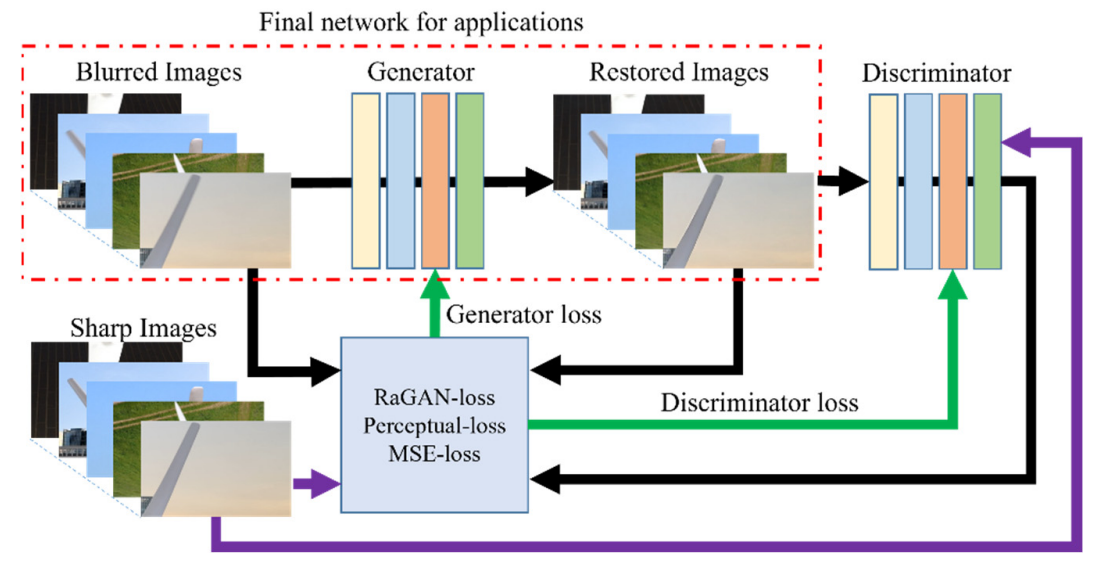
\includegraphics[width=15cm]{Images/turbinablur.png}
        \caption{Flowchart of DeblurGANv2-based motion deblurring of wind turbine blade images. \cite{TurbineBlur}}
        \label{fig:TurbinaDiagrama}
    \end{figure}

    \cite{BlenderSmoke} used a Faster R-CNN network to detect forest fire smoke, overcoming the sparsity of suitable smoke images by generating two synthetic datasets: one with real smoke filmed against a green screen and composited onto landscape footage, and another with smoke rendered entirely in Blender.
    The model trained on Blender-rendered smoke outperformed the one trained on composited real smoke, demonstrating that fully synthetic data can achieve superior results when the rendering pipeline adequately captures the visual characteristics of the target phenomenon.

    \cite{ObjetoSintetico} tackled the scarcity of labeled image data for food package detection in refrigerators.
    The authors produced a fully synthetic bank of 4,000 Blender-rendered images and a hybrid bank combining 3,600 synthetic images with 400 real images.
    Training a GoogleNet Fully Convolutional network for 200 epochs, the hybrid dataset achieved a mAP of 36, outperforming both the synthetic-only (mAP 24) and real-only (mAP 28) configurations, reinforcing the value of mixing synthetic and real data.

    \cite{BlenderMapa} created three-dimensional environments in Blender to generate image samples at distinct poses for mobile device pose estimation.
    A PoseNet network based on GoogLeNet with 23 layers and six inception modules was trained on these synthetic images, achieving localization accuracy of approximately 2 meters in real time.

    The synthetic data strategy adopted in the present work follows the same principles, with the critical difference that the target domain of water surfaces, presents unique rendering challenges related to physically-based wave modeling, subsurface scattering, and view-dependent specular behavior, which were addressed through Blender's ocean modifier and physically-based shading pipeline.
    The domain randomization principles established by \cite{Tobin2017} and \cite{Tremblay2018} further support this approach, showing that variability in synthetic rendering parameters can improve generalization to real-world conditions.

    \subsection{Broader Applications and Future Directions}

    The altitude estimation capability developed in this work has potential implications beyond the immediate application of single-UAV flight control.
    \cite{XuMicroUAVSwarm2025} introduced a comprehensive micro-UAV swarm system for indoor perception in partially known environments, proposing integrated solutions for communication routing, multisensor localization, and cooperative decision-making.
    Swarm systems of this nature demands that each individual UAV maintain reliable altitude estimation with minimal computational overhead, as the processing budget must be shared across navigation, communication, and coordination tasks.
    A lightweight, vision-based altitude estimator such as the one proposed here could serve as a complementary sensor for swarm members operating over water, where traditional altimetry is unreliable and the weight and power constraints of micro-UAVs preclude the addition of dedicated ranging hardware.

    The convergence of these research directions, regard CNN-based metric estimation, water surface perception, synthetic data generation, and swarm UAV architectures, defines the space in which the present work makes its contribution: a problem that is simultaneously well-motivated by practical needs and inadequately addressed by existing methods.